	\subsection{Démarche entretenue}
Afin de répondre à notre problématique, nous avons décidé de mettre en place une \textbf{application web} qui interroge une \textbf{base de donnée} contenant les mesures des différents patients. 
Nous avons alors réalisé une première page d'identification pour se connecter à ce web-service. 
En effet, cela touchant des données médicales, il faut que les données soient un minimum protégées. 
Ensuite, nous avons réalisé une seconde page qui récupère la liste des personnes ayant pris des mesures et affiche un \textbf{formulaire de sélection} permettant de choisir la session du patient dont on veut consulter les données. 
Une fois validé, cette page envoie une requête à un web-service qui va interroger la base de donnée permettant d'aller chercher les différentes mesures relatives a la session choisie, s'affichant alors sur la troisieme page web. \\
Nous avons alors choisis de traiter ces données en suivant un arbre de décision (\textit{image ci-dessous}), afin de renvoyer une indication pour un éventuel diagnostique pour un médecin. 


	\subsection{Arbre de decision}
\begin{figure}[h]
    \centerline{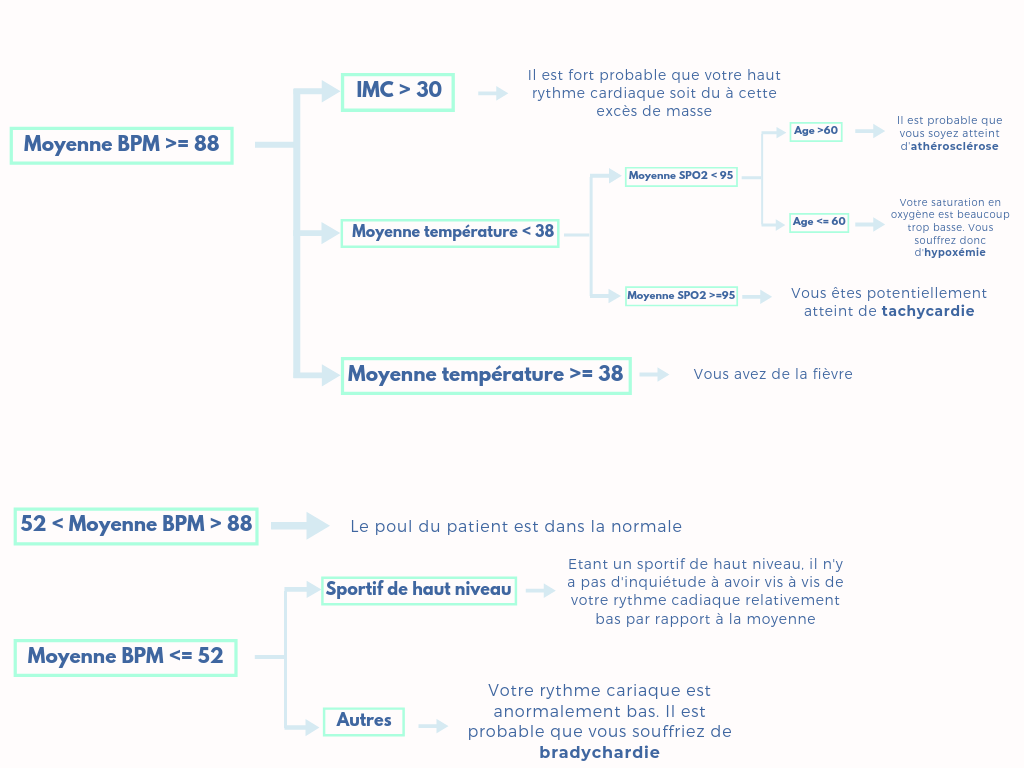
\includegraphics[width=16cm, height=10cm]{arbre.png}}
\end{figure}
\newpage

Nous avons choisi de traiter "3 types de patients" :
\begin{itemize}
\item Patient avec un BPM inférieur à 52 (Patient dans le 5ème percentile)
\item Patient avec un BPM entre 52 et 88 (Patient entre le 10ème et le 90ème percentile)
\item Patient avec un BPM supérieur à 88 (Patient dans le 95ème percentile)
\end{itemize} 
Ce classement s'est effectué selon une étude canadienne certifiée HON et correspond aux moyennes selon une étude sur la population.
On s'intéresse donc pour chacun de ces cas, à ce qui pourrait influencer le rythme cardiaque.
\textit{Par exemple}, nous avons analysé l'\textit{Indice de Masse Corporel} (IMC) qui permet d'évaluer la corpulence d'un individu en tenant compte uniquement de sa taille et de son poids. Cet indice permet de déterminer si une personne est en surpoids. En effet, une personne en surpoids ou obésité aura un rythme cardiaque plus élevé qu'un autre.
\\
Ainsi, grâce à tous les paramètres que nous possédons (taille, age, sexe, activité sportive, température, BPM, saturation en O2, ...), nous avons pu établir un premier avis permettant d'aider le médecin dans la détection d'un trouble cardiaque.
